\documentclass[a4paper,12pt]{article}
% -------------------------------------------------------------------
%                  Essential packages (used in template)
% -------------------------------------------------------------------

\usepackage[utf8]{inputenc}                   % Allow Umlauts (ä, ö, ü)
\usepackage[ngerman]{babel, translator}       % German LaTeX-intern descriptors (Abbildungen, ...)
\usepackage{mathptmx}                         % Font "Times New Roman" in mathematical Environments
\usepackage{courier}                          % Support the use of font "Courier" (used in listings)
\usepackage[T1]{fontenc}                      % Change LaTeX font encoding to support modern fonts
\usepackage{fix-cm}                           % Fix sizes at which CM and EC fonts can be used

\usepackage{geometry}                         % Change text bounds on a per-page basis
\usepackage{fancyhdr}                         % Allow easy customization of headers and footers

\usepackage[ddmmyyyy]{datetime}               % Reformat times from LaTeX commands like \today

\usepackage[dvipsnames]{xcolor}               % Support text colorization

\usepackage{colortbl}                         % Support applying colors to tables
\usepackage{array}                            % Tables with fixed column size
\usepackage{longtable}                        % Support multi-page tables
\usepackage{multicol}                         % Additional settings for \multicolumn
\usepackage{multirow}                         % Additional settings for \multirow

\usepackage[hyphens,obeyspaces,spaces]{url}   % Allow urls to have line breaks at "-"
\usepackage{microtype}                        % Enable "Blocksatz"

\usepackage{float}                            % Support for table H option
\usepackage{floatflt}                         % Support text wrapping around floating environments
\usepackage{wrapfig}                          % Support text wrapping around figures

\usepackage{graphicx}                         % Support including graphics environments for images
\usepackage{caption}                          % Provide greater customization around captions
\usepackage{subcaption}                       % Caption support for subfigures
\usepackage{pdfpages}                         % Include existing PDFs into the work

\usepackage[onehalfspacing]{setspace}         % Set line spacing to be 1.5x the default
\usepackage{listings}                         % Code block support for LaTeX

\usepackage[titles]{tocloft}                  % More options to modify list of figures & tables
\usepackage{nomencl}                          % Support for nomenclatures ("Symbolverzeichnis")

\usepackage{amsmath}                          % Includes a plethora of mathematical packages 
\usepackage{amssymb}                          % Source mathematical symbols like \sin
\usepackage{amsthm}                           % Better theorems
\usepackage{upgreek}                          % Use \Upomega to get a straight \Omega
\usepackage{siunitx}                          % Unified support for si units

\usepackage{ifthen}                           % Support better if statements in LaTeX
\usepackage{etoolbox}                         % Easily patch commands

\usepackage{hyperref}                         % Clickable hyperlinks in Table of Contents

% Support list of acronyms and glossary
\usepackage[
  toc,
  nogroupskip,
  nonumberlist,
  nopostdot,
  acronyms,
  shortcuts,
  translate=babel
]{glossaries}

% Track the total count of different environments
% Needs to be imported because LaTeX resets these counter on a chapter basis
\usepackage[figure,table,lstlisting,xspace]{totalcount}

% Annotate different information directly into the document
\setlength{\marginparwidth}{2cm}
\usepackage[
  colorinlistoftodos,
  prependcaption,
  textsize=tiny
]{todonotes}

% -------------------------------------------------------------------
%                 Useful packages (not used in template)
% -------------------------------------------------------------------

% Create electrical diagrams from within LaTeX
\usepackage[
  european,
  oldvoltagedirection,
  straightvoltages,
  siunitx
]{circuitikz}

% Annotate images with standard tikz macros
\usepackage{tikz-imagelabels}

% Disable single lines at the start of a paragraph (Schusterjungen)
\clubpenalty=10000

% Disable single lines at the end of a paragraph (Hurenkinder)
\widowpenalty=10000
\displaywidowpenalty=10000

% Fixed size table columns
\newcolumntype{L}[1]{>{\raggedright\arraybackslash}p{#1}}
\newcolumntype{C}[1]{>{\centering\arraybackslash}p{#1}}
\newcolumntype{R}[1]{>{\raggedleft\arraybackslash}p{#1}}

\renewcommand{\arraystretch}{1.2}                       % Distance between lines in tables

\captionsetup{justification=raggedright}                % Align captions to the left

\setcounter{secnumdepth}{3}                             % Only allow nesting 3 layers (down to subsubsections)

% Unit-related setup for siunitx
\sisetup{
  locale=DE,                   % Use German notation (comma instead of point delimiter for floats)
  per-mode=fraction,           % Switch display to use \frac instead of x^{-1}
  fraction-function=\tfrac,    % Use amsmath's tfrac macro for unit fractions
}

% -------------------------------------------------------------------
%                     Usability & visual changes
% -------------------------------------------------------------------

% Page margins
\geometry{
  left=2.5cm,
  right=2.5cm,
  top=2.5cm,
  bottom=3cm
}

% Create a better looking header and footer
\pagestyle{fancy}
\fancyhf{}
\lhead{\nouppercase{\leftmark}}
\rfoot{\thepage}

% Automatically generate a box around figure environments
\floatstyle{boxed}
\restylefloat{figure}

% Set toc sections to be clickable
\hypersetup{
  colorlinks,
  citecolor=black,
  filecolor=black,
  linkcolor=black
}

\frenchspacing                                                 % Insert one space after a sentence, not 2

\renewcommand{\theequation}{\thesection.\arabic{equation}}     % Numbering of equation schould be x.x
\renewcommand{\UrlFont}{\color{blue}\rmfamily\itshape}         % URLs should be displayed in blue
\renewcommand{\dateseparator}{.}                               % Dates are written like 01.01.1970, not 01-01-1970

\addto{\captionsngerman}{
  \renewcommand*{\figurename}{Abb.}                            % Figures should be displayed as "Abb. x"
  \renewcommand*{\tablename}{Tab.}                             % Tables  should be displayed as "Tab. x"
  \renewcommand*{\lstlistingname}{Code}                        % Code    should be displayed as "Code x"
  %
  \renewcommand*{\lstlistlistingname}{Codebeispielverzeichnis} % List of listings
  \renewcommand*{\nomname}{Symbolverzeichnis}                  % Nomenclature
  \renewcommand*{\acronymname}{Abkürzungsverzeichnis}          % List of acronyms
  \renewcommand*{\refname}{Literaturverzeichnis}               % Bibliography
  %
  \providecommand{\declarationname}{}
  \renewcommand*{\declarationname}{Ehrenwörtliche Erklärung}   % Declaration of honor
}

\addto{\extrasngerman}{%
  \def\sectionautorefname{Kapitel}%                              1st level sections should be called "Kapitel"
  \def\subsectionautorefname{Abschnitt}%                         2nd level sections should be called "Abschnitt"
  \def\subsubsectionautorefname{Unterabschnitt}%                 3rd level sections should be called "Unterabschnitt"
}

% -------------------------------------------------------------------
%                        Code listing setup
% -------------------------------------------------------------------

\lstset{
  basicstyle=\small\ttfamily\color{black},              % Font size used for the code
  commentstyle=\ttfamily\color{gray},                   % Comment style
  keywordstyle=\ttfamily\color{blue},                   % Keyword style
  stringstyle=\color{ForestGreen!30!LimeGreen},         % String literal style
  frame=single,                                         % Add a frame around the code
  showstringspaces=false,                               % Don't underline spaces within strings only
  captionpos=b,                                         % Set caption-position to bottom
  backgroundcolor=\color{white},                        % Background color
}

% To style lstlistlisting like the lof, you first have to register it
% to tocloft, as mentioned in https://tex.stackexchange.com/a/27648/27635
\makeatletter
\begingroup\let\newcounter\@gobble\let\setcounter\@gobbletwo
  \globaldefs\@ne \let\c@loldepth\@ne
  \newlistof{listings}{lol}{\lstlistlistingname}
\endgroup
\let\l@lstlisting\l@listings
\makeatother

% -------------------------------------------------------------------
%                         Redefining geometry
% -------------------------------------------------------------------

% Figures
\renewcommand{\cftfigpresnum}{\figurename~}
\renewcommand{\cftfigaftersnum}{:}
\setlength{\cftfignumwidth}{2cm}
\setlength{\cftfigindent}{0cm}

\AtBeginEnvironment{figure}{\vspace{1em}}               % Increase spacing of images from the text above

% Tables
\renewcommand{\cfttabpresnum}{\tablename~}
\renewcommand{\cfttabaftersnum}{:}
\setlength{\cfttabnumwidth}{2cm}
\setlength{\cfttabindent}{0cm}

% Listings
\renewcommand*{\cftlistingspresnum}{\lstlistingname~}
\renewcommand*{\cftlistingsaftersnum}{:}
\settowidth{\cftlistingsnumwidth}{\cftlistingspresnum}
\addtolength{\cftlistingsnumwidth}{1cm}
\setlength{\cftlistingsindent}{0cm}

\setlength{\parindent}{0cm}                             % Don't indent start of paragraph
\setlength{\parskip}{6pt}                               % Lines are separated by 6pt

\setlength{\headheight}{1.25cm}
\setlength{\footskip}{1cm}
\setlength{\headsep}{1cm}

% -------------------------------------------------------------------
%                    Custom counters & commands
% -------------------------------------------------------------------

% Custom acronym patches:
%   - count usage (used for on-demand list of acronyms)
%   - provide shorter aliases for commonly used macros
\newcounter{countacronym}
\DeclareTotalCounter{countacronym}
\pretocmd{\acrshort}{\stepcounter{countacronym}}{}{}
\pretocmd{\acrlong}{\stepcounter{countacronym}}{}{}
\pretocmd{\acrfull}{\stepcounter{countacronym}}{}{}
\newcommand*{\acr}[1]{\acrshort{#1}}
\newcommand*{\Acr}[1]{\acrlong{#1}}

% Custom nomenclature patches:
%   - count usage of actual entries through \nomen (used for on-demand nomenclature)
%   - provide cleaner writing interface with pre-made abstractions
\newcounter{countnomen}
\DeclareTotalCounter{countnomen}
\newcommand*{\nomen}[2]{\nomenclature{#1}{#2}\stepcounter{countnomen}}
\newcommand{\nomunit}[1]{\renewcommand{\nomentryend}{\hspace*{\fill}#1}}
\newcommand{\nomsi}[1]{\nomunit{[\si{#1}]}}

% Custom glossary patches:
%   - count usage (used for on-demand glossary)
\newcounter{countglossary}
\DeclareTotalCounter{countglossary}
\pretocmd{\Gls}{\stepcounter{countglossary}}{}{}
\pretocmd{\gls}{\stepcounter{countglossary}}{}{}
\pretocmd{\Glspl}{\stepcounter{countglossary}}{}{}
\pretocmd{\glspl}{\stepcounter{countglossary}}{}{}

% Custom citation patches:
%   - count usage (used for on-demand bibliography)
\newcounter{countcitation}
\DeclareTotalCounter{countcitation}
\pretocmd{\cite}{\stepcounter{countcitation}}{}{}

% TODO annotations
\newcounter{counttodo}
\DeclareTotalCounter{counttodo}
\pretocmd{\todo}{\stepcounter{counttodo}}{}{}
\newcommand{\note}   [2][]{\todo[color=green!25,bordercolor=green,tickmarkheight=3pt,#1]{#2}}
\newcommand{\unsure} [2][]{\todo[color=Plum!25,bordercolor=Plum,tickmarkheight=3pt,#1]{#2}}
\newcommand{\change} [2][]{\todo[color=blue!25,bordercolor=blue,tickmarkheight=3pt,#1]{#2}}
\newcommand{\missing}[2][]{\todo[color=red!25,bordercolor=red,tickmarkheight=3pt,#1]{#2}}
\newcommand{\info}   [2][]{\todo[nolist,color=yellow!25,bordercolor=yellow,tickmarkheight=3pt,#1]{#2}}

% Larger clickable references to page items
\newcommand{\imgref} [1]{\hyperref[#1]{Abbildung~\getrefnumber{#1}}}
\newcommand{\tabref} [1]{\hyperref[#1]{Tabelle~\getrefnumber{#1}}}
\newcommand{\coderef}[1]{\hyperref[#1]{Code~\getrefnumber{#1}}}
\newcommand{\mathref}[1]{\hyperref[#1]{Gleichung~\getrefnumber{#1}}}
\newcommand{\secref} [1]{\autoref{#1}}


% Preload custom user settings & packages
\IfFileExists{./Custom.tex}{\usepackage{graphicx}
\usepackage{caption}
\usepackage{subcaption}}{}

% ===========================================================================
%           Wrap document environment with HSCDocument environment
% ===========================================================================

\AddToHook{env/HSCDocument/before}{

  % Register different entries: glossary, nomenclature, acronyms
  \makeglossaries
  \hyphenation{}

  \newacronym{EUT}{EUT}{Expected-Utility-Theorie}
  \makenomenclature
  \nomenclature[01]{\textbf{Symbol}}{\textbf{Bedeutung} \nomunit{\textbf{[phys. Einheit]}}}

  \newglossaryentry{Glossar}
{
    name=Glossar,
    plural=Glossare,
    description={"selbstständig oder als Anhang eines bestimmten Textes erscheinendes Wörterverzeichnis" \cite{Duden}}
}

  \begin{document}
}

\AddToHook{env/HSCDocument/after}{
  \end{document}
}

\makeatletter
\define@key{HSCDocument@keys}{preset}{\def\DocumentType{#1}}
\makeatother

\newenvironment{HSCDocument}[1][]{

  \makeatletter
  \setkeys{HSCDocument@keys}{
    preset=Custom,
    #1
  }
  \makeatother

  % Don't display "a as ä etc.
  \shorthandoff{"}

  % ===========================================================================
  %                             Document header
  % ===========================================================================

  \newgeometry{
    left=2.5cm,
    right=2.5cm,
    top=2.5cm,
    bottom=2.5cm
  }

  \begin{titlepage}
    \ifthenelse{\equal{\DocumentType}{Praxisbericht}}
      {\centering

\includegraphics[width=.8\textwidth]{framework/Logo_HS_Coburg}

\begin{Large}
  Hochschule für angewandte Wissenschaften Coburg\\
  Fakultät Elektrotechnik und Informatik\par
\end{Large}
\vspace{1.5cm}

\Large{Studiengang: \Studiengang}
\vspace{1.5cm}

\Large{Praxisbericht}
\vspace{1cm}

\huge{\Autorenname}
\vspace{1.5cm}

\begin{table}[H]
  \begin{tabular}{|L{3cm}|L{11cm}|}
  \hline
  Unternehmen & \Unternehmen        \\
              & \Abteilung          \\
              & \Strasse            \\
              & \Ort                \\
  \hline
  Zeitraum    & \Beginn \ bis \Ende \\
  \hline
  \end{tabular}
\end{table}

\large{Abgabe des Berichts: \Abgabe}

\begin{table}[H]
  \begin{tabular}{|L{3cm}|L{6cm}|L{5cm}|}
    \multicolumn{3}{l}{Freigabe zur Vorlage des Praxisberichts an der HS Coburg:} \\
    \hline
    Betreuer & \Betreuer & \\
    \hline
    Funktion & \Funktion & \textbf{\textit{Ort, Datum}}\\
    \hline
    Telefon & \Telefon & \\
    \cline{1-2}
    Email & \Email & \\
    \hline
    & & \textbf{\textit{Unterschrift Betreuer}}\\
    \hline
  \end{tabular}
\end{table}
}
      {
        \ifthenelse{\equal{\DocumentType}{Bachelorarbeit}}
          {\centering

\includegraphics[width=.8\textwidth]{framework/Logo_HS_Coburg}

\begin{Large}
  Hochschule für angewandte Wissenschaften Coburg\\
  Fakultät Elektrotechnik und Informatik\par
\end{Large}
\vspace{1.5cm}

\Large{Studiengang: \Studiengang}
\vspace{1.5cm}

\Huge{\Titel}
\vspace{2cm}

\huge{\Autorenname}
\vspace{2cm}

\Large{Abgabe der Arbeit: \Abgabe}

\Large{Betreut durch:}

\Large{\Dozent, Hochschule Coburg}
}
          {
            \ifthenelse{\equal{\DocumentType}{Masterarbeit}}
              {\centering

\includegraphics[width=.8\textwidth]{framework/Logo_HS_Coburg}

\begin{Large}
  Hochschule für angewandte Wissenschaften Coburg\\
  Fakultät Elektrotechnik und Informatik\par
\end{Large}
\vspace{1.5cm}

\Large{Studiengang: \Studiengang}
\vspace{1.5cm}

\Huge{\Titel}
\vspace{2cm}

\huge{\Autorenname}
\vspace{2cm}

\Large{Abgabe der Arbeit: \Abgabe}

\Large{Betreut durch:}

\Large{\Dozent, Hochschule Coburg}
}
              {
                \IfFileExists{./CustomHeader.tex}{
                  \include{CustomHeader}
                }{
                  ERROR: Please use one of the following values as parameter
                  to the HSCdocument environment:\\
                  "Praxisbericht", "Bachelorarbeit", "Masterarbeit"\\

                  To create your own document header, just create a file
                  "CustomHeader.tex" in the document root.
                }
              }
          }
      }
  \end{titlepage}

  \restoregeometry

  % Header is considered the 1st page
  \addtocounter{page}{1}

  % ===========================================================================
  %                              Page Ordering
  % ===========================================================================

  % Set image path to "Bilder" subdirectory
  \graphicspath{{Bilder/}}

  % Optional notice to the reader ("Vermerk")
  \IfFileExists{./Sektionen/Vermerk.tex}{
    \newpage
    \thispagestyle{empty}
    \include{Sektionen/Vermerk}
  }{}

  % Abstract
  \IfFileExists{./Sektionen/Abstract.tex}{
    \newpage
    \fancypagestyle{abstract}{
      \fancyhead[L]{Abstract}
    }
    \thispagestyle{abstract}
    \include{Sektionen/Abstract}
  }{}

  \newpage
  \tableofcontents

  \iftotalfigures
    \newpage
    \phantomsection
    \addcontentsline{toc}{section}{\listfigurename}
    \listoffigures
  \fi

  \iftotaltables
    \newpage
    \phantomsection
    \addcontentsline{toc}{section}{\listtablename}
    \listoftables
  \fi

  \iftotallstlistings
    \newpage
    \phantomsection
    \addcontentsline{toc}{section}{\lstlistlistingname}
    \lstlistoflistings
  \fi

  % Nomenclature ("Symbolverzeichnis")
  \iftotalcountnomens
    \newpage
    \phantomsection
    \addcontentsline{toc}{section}{\nomname}
    \printnomenclature[1in]
  \fi

  % Acronyms
  \iftotalcountacronyms
    \newpage
    \setglossarystyle{super}
    \printglossary[type=\acronymtype]
  \fi

  \newpage
}
{
  % Bibliography
  \iftotalcountcitations
    \newpage
    \bibliographystyle{alphadin}
    \phantomsection
    \addcontentsline{toc}{section}{\refname}
    \bibliography{Verzeichnisse/Literaturverzeichnis}
  \fi

  % Glossary
  \iftotalcountglossarys
    \newpage
    \setglossarystyle{altlist}
    \printglossary
  \fi

  % Appendix
  \IfFileExists{./Sektionen/Anhang.tex}{
    \newpage
    \appendix
    \renewcommand{\thesection}{A\arabic{section}}
    \include{Sektionen/Anhang}
  }{}

  % Declaration of Honor
  \newpage
  \phantomsection
  \addcontentsline{toc}{section}{\declarationname}
  \lhead{\declarationname}
  \thispagestyle{empty}

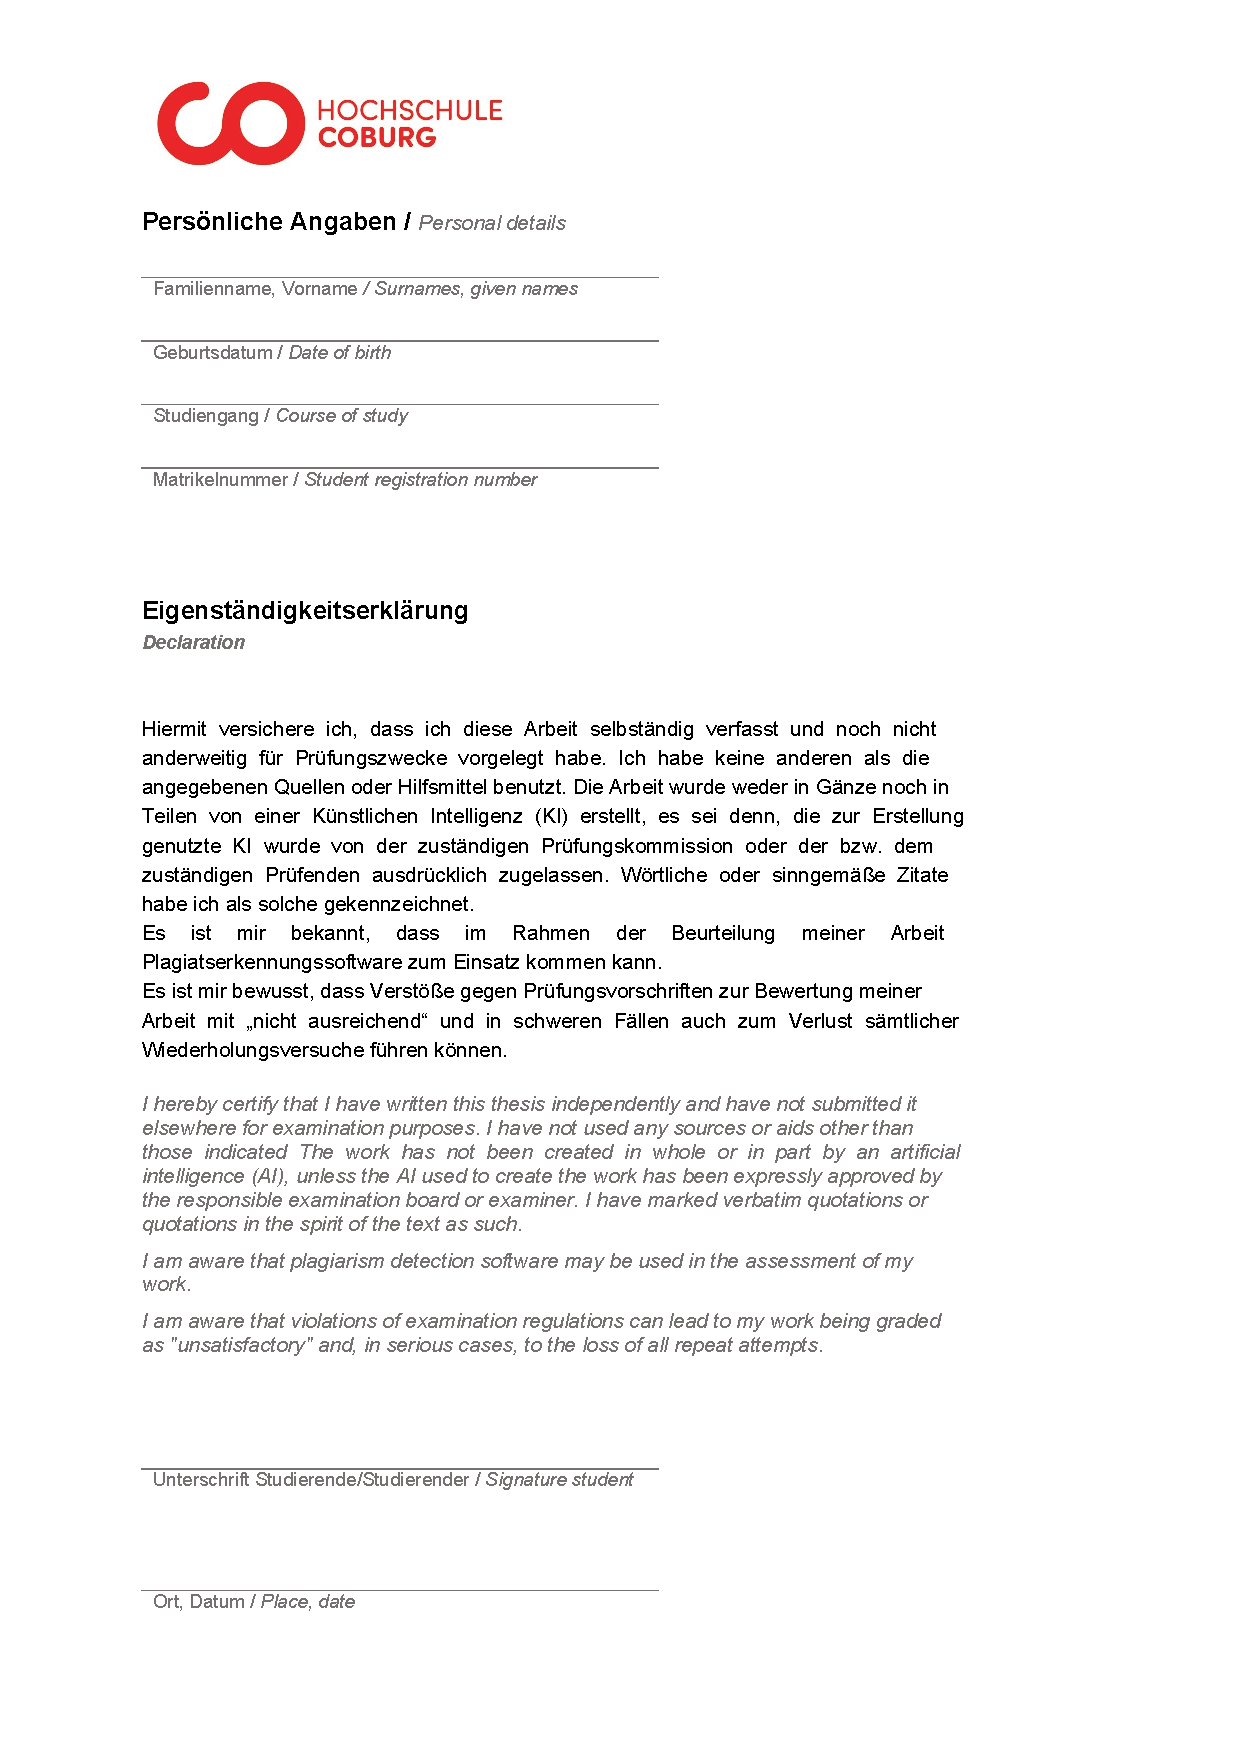
\includepdf[
  pages=-,
  pagecommand={},
  picturecommand*={
    \put(75,714){\large \Autorenname}
    \put(75,683){\large \Geburtsdatum}
    \put(75,652){\large \Studiengang}
    \put(75,622){\large \Matrikelnummer}
    \put(75,81.5){\large \Ort, den \today}
  }
]{framework/_Declaration_of_Honor.pdf}


  % TODO list
  \iftotalcounttodos
    \phantomsection
    \addcontentsline{toc}{section}{TODOs}
    \thispagestyle{empty}
    \listoftodos[TODOs]
  \fi
}

% ===========================================================================
%                   Simplified centered & colored tables
% ===========================================================================

\newenvironment{colortable}[1]{
  \begin{center}
    \begin{tabular}{#1}
    \hline
    \rowcolor{Gray}
}
{
    \hline
    \end{tabular}
  \end{center}
}

\newcommand{\tablecontent}{
  \hline
  \rowcolor{White}
}


\def\Titel{Vorlage für verschiedene Dokumente der HS Coburg}
\def\Dozent{<DOZENT>}

% Infos zum Autor
\def\Autorenname{<NACHNAME, VORNAME>}
\def\Geburtsdatum{<GEBURTSDATUM>}
\def\Matrikelnummer{<MATRIKELNUMMER>}
\def\Studiengang{<STUDIENGANG>}

% Infos zum Unternehmen
\def\Unternehmen{<FIRMENNAME>}
\def\Abteilung{<ABTEILUNG>}
\def\Strasse{<STRAßE>}
\def\Ort{<ORT>}

% Infos zum Betreuer
\def\Betreuer{<BETREUER>}
\def\Funktion{<FUNKTION BETREUER>}
\def\Telefon{<TELEFONNUMMER BETREUER>}
\def\Email{<BETREUER EMAIL>}

% Daten
\def\Beginn{<BEGINN>}
\def\Ende{<ENDE>}
\def\Abgabe{\today}

\begin{HSCDocument}[preset=Praxisbericht]

  \section{Einleitung}
Ein fundamentales Konzept in den Wirtschaftswissenschaften ist die von Frank H. Knight eingeführte Unterscheidung zwischen Risiko und 
Unsicherheit. Knight definierte Risiko als quantifizierbare Unsicherheit, also Situationen, in denen den möglichen Ergebnissen 
Wahrscheinlichkeiten zugeordnet werden können. Ein klassisches Beispiel hierfür sind Versicherungen oder Glücksspiele, bei denen 
aufgrund historischer Daten oder mathematischer Modelle die Wahrscheinlichkeiten der verschiedenen Ausgänge bekannt sind.

Unsicherheit hingegen, die Knight als "echte Unsicherheit" bezeichnet, bezieht sich auf Situationen, in denen diese Zuordnung nicht 
möglich ist. Dies tritt auf, wenn keine verlässlichen historischen Daten zur Verfügung stehen, um die Wahrscheinlichkeiten der 
verschiedenen Ergebnisse zu prognostizieren. Ein Beispiel hierfür wäre die Einführung eines innovativen Produkts auf den Markt, bei 
dem es keine vorherigen Daten gibt, die den Erfolg oder Misserfolg vorhersagen könnten. \cite{Knight1921}

Wenn man Unsicherheit aus der Perspektive der Datenvisualisierung betrachtet, stößt man auf viele ähnliche, jedoch auch zahlreiche 
unterschiedliche Definitionen. Haber und McNabb \cite{Haber1990} beschreiben einen generischen Prozess zur Visualisierung von Daten, 
der die verschiedenen Stufen von der Datenbeschaffung bis zur finalen Visualisierung abdeckt. Dieser Prozess, der auch von Pang et al. \cite{Pang1997} 
aufgegriffen wird, besteht aus mehreren Schritten, in denen Unsicherheit in unterschiedlichem Maße eingeführt und berücksichtigt
werden muss, und diese unterschiedlichen Definitionen verdeutlicht:

\begin{enumerate}
    \item \textbf{Datenbeschaffung}:
    In dieser Phase ist Unsicherheit inherent, sei es durch Messfehler/-ungenauigkeiten, die Beschaffung der Daten durch statistische Modelle oder unvollständige Daten.
    
    \item \textbf{Datenvorverarbeitung}:
    Die beschafften Daten müssen in einem nachgehenden Schritt aufbereitet werden, in welchem durch Interpolation von fehlenden Daten, ungenaue Transformationen oder Annahmen weitere Unsicherheit einfließen kann.
    
    \item \textbf{Datenverarbeitung und -analyse}:
    Diese Daten werden zur Visualisierung auf ein/mehrere geometrische Objekte gemappt. Dies stellt durch die verwendeten Algorithmen und Modelle eine neue Quelle von Unsicherheit dar.
    
    \item \textbf{Visualisierung}:
    Schließlich werden die Daten visualisiert. Hier können Unsicherheiten durch die Wahl der Visualisierungstechniken und Darstellungsparameter wie Farbskalen und Fehlerbalken an sich beeinflusst werden.
\end{enumerate}

\subsection{Die Bedeutung von Unsicherheit in Finanzmärkten}
Knight schrieb in seinem Werk ausserdem, dass in einem fairen Markt nur ein Unternehmer wirtschaftlich erfolgreich
sein kann, wenn dieser Unsicherheiten auf sich nimmt, da andernfalls jeder Marktteilnehmer die gleichen, korrekten 
Informationen hätte und somit kein Vorteil erarbeitet werden kann.
Wird diese aufzunehmende Unsicherheit aber im Entscheidungsprozess falsch oder unzureichend dargestellt, kann dies fatale Folgen nach sich 
ziehen. 

Man stelle sich beispielsweise die Prognose eines Aktienkurses anhand eines Monte-Carlo-Modells vor. Sollte ein Investor auf Basis 
dieser Prognose eine Entscheidung treffen, ist er einerseits mit der direkten quantitativen Unsicherheit der Vorhersage konfrontiert, 
also mit der Wahrscheinlichkeit, dass genau der gewählte Zweig der Simulation zutrifft, und der Varianz. Andererseits gibt es die 
indirekte qualitative Unsicherheit: Hat der Ersteller korrekt historische Daten verwendet? \cite{Padilla2021} Auf welcher Basis von Zufall wurde die Prognose erstellt –
Volatilität oder fundierte ökonomische Kennzahlen des Unternehmens? Es gilt, diese Unsicherheiten so gut wie möglich darzustellen, 
um den Investor bei seiner Entscheidungsfindung zu unterstützen und keine Trugschlüsse zuzulassen.

\subsection{Ziele der Arbeit}
Deshalb wird in dieser Arbeit untersucht, wie sich die Visualisierung von Unsicherheiten und Risiken auf Entscheidungsträger auswirkt, wie Techniken angewandt werden können um 
die Kommunikation von Information zwischen Laien und professionellen verbessert werden kann und wie bereits entwickelte Techniken aus anderen Domänen auf die Finanzwelt übertragen werden können.

Im folgendem Kapitel werden Grundlagen zur Entscheidungsfindungen von Menschen sowie Techniken der Visualisierung von Unsicherheiten beleuchtet,
daraufhin


\section{Theoretische Grundlagen}
Es wird die Basis geschaffen um Visualiserungstechniken sowie ihre Bedeutung in der Entscheidungsfindung besser verstehen zu können.

\subsection{Theorien zur Entscheidungsfindung unter Unsicherheit}
Im Folgendem werden Theorien zur Entscheidungsfindung unter Unsicherheit näher beleuchtet, welche laut Padille et al. notwendigerweiße berücksichtigt
werden müssen, um Visualisierungstechniken auf Basis ihrer Rolle in Entscheidungsfindungen in anbetracht von Unsicherheit bewerten zu können. Diese 
werden in Sektion 3 wieder aufgegriffen, um die Auswirkung unterschiedlicher Visualisierungsmethoden auf die Entscheidungsfindung zu erklären. \cite{VisualizationPsychology2023}

\subsubsection{Erwartungsnutzentheorie}

Die Erwartungsnutzentheorie (\ac{EUT}) ist ein grundlegendes Modell in der Entscheidungstheorie, das beschreibt, wie rationale Akteure Entscheidungen unter Unsicherheit 
treffen sollten. Entwickelt von John von Neumann und Oskar Morgenstern, basiert die EUT auf der Annahme, dass Individuen bei der 
Wahl zwischen unsicheren Alternativen jene Option bevorzugen, die den höchsten erwarteten Nutzen bietet. Der erwartete Nutzen eines 
Ergebnisses wird dabei als das Produkt aus der Wahrscheinlichkeit des Ergebnisses und dem subjektiven Wert (Nutzen) dieses Ergebnisses 
berechnet.

Die formale Darstellung der Erwartungsnutzentheorie lautet:

\begin{equation}
EU = \sum_{i=1}^{n} p_i \cdot u(x_i)
\end{equation}

Dabei ist \( EU \) der erwartete Nutzen, \( p_i \) die Wahrscheinlichkeit des Ergebnisses \( x_i \) und \( u(x_i) \) der Nutzen des 
Ergebnisses \( x_i \).

Die EUT geht davon aus, dass Individuen konsistente Präferenzen haben und stets die Alternative mit dem höchsten erwarteten Nutzen 
wählen. \cite{vonNeumann1944} Diese Theorie hat weitreichende Anwendungen in der Finanzwelt, beispielsweise bei der Analyse von 
Investitionsentscheidungen und Risiken. 

\subsubsection{Dual-Process-Theorie}

Die Dual-Process-Theorie beschreibt, wie Menschen zwei verschiedene Arten von Denkprozessen nutzen, um Entscheidungen zu treffen: 
intuitives (Type 1) und analytisches (Type 2) Denken. Fundierungen für diese Theorie wurden von Psychologen wie Daniel Kahneman und Keith 
Stanovich zum Beispie in \cite{Tversky74} über Jahre hinweg entwickelt und hebt hervor, dass Menschen je nach Situation und 
Komplexität der Aufgabe zwischen diesen beiden Denkmodi wechseln.

\begin{itemize}
    \item \textbf{Type 1 Prozesse}: Diese sind schnell, automatisch und erfordern wenig kognitive Anstrengung. 
    Sie basieren auf Intuition und Heuristiken, die oft aus Erfahrungen und erlernten Mustern resultieren. 
    Type 1 Prozesse sind nützlich in routinierten und vertrauten Situationen, können jedoch zu systematischen 
    Fehlern und Verzerrungen führen.
    \item \textbf{Type 2 Prozesse}: Diese sind langsam, bewusst und erfordern erhebliche kognitive Anstrengung. 
    Sie basieren auf logischem Denken und systematischer Analyse. Type 2 Prozesse kommen zum Einsatz, wenn komplexe 
    und neue Situationen eine gründliche Bewertung erfordern.
\end{itemize}

Die Dual-Process-Theorie erklärt, warum Menschen in vielen Situationen intuitive Entscheidungen treffen, die schnell und effizient 
sind, aber manchmal zu suboptimalen Ergebnissen führen. Sie betont auch die Notwendigkeit, analytisches Denken zu fördern, 
insbesondere bei komplexen und wichtigen Entscheidungen, bei denen Fehler schwerwiegende Konsequenzen haben können.


\subsection{Hintergrundwissen zur Visualisierung von Unsicherheit}

Um die Bedeutung der Visualisierung von Unsicherheiten auf die Entscheidungsfindung besser zu verstehen, werden hier
Konzepte und Techniken erläutert, welche bekanntermassen eine positive Auswirkung auf die rationale Entscheidungsfindung haben, 
was in Sektion 3 weiter beleuchtet wird.

\subsubsection{Quantile Dotplots}
Quantile Dotplots sind eine Visualisierungstechnik, die darauf abzielt, Unsicherheit durch diskrete Punkte darzustellen, 
die bestimmte Quantile einer Verteilung repräsentieren. Diese Methode hilft den Nutzern, Wahrscheinlichkeiten und Verteilungen 
auf intuitive Weise zu verstehen, indem sie visuelle Hinweise liefert, die leicht gezählt und interpretiert werden können. 
Kay et al. haben gezeigt, dass Quantile Dotplots die Genauigkeit von Entscheidungsfindungen verbessern können, indem sie die 
Verteilung von Unsicherheiten klar und verständlich darstellen. \cite{Kay2016}.

Diese Technik schneidet nicht nur in normalen Bewertungsmaßen 
von Visualiesierungsmethoden, nämlich wie akkurat und schnell sie Informationen übermitteln können, gut ab, sonder verbessern
nach Fernandes et al. auch die Fähigkeit rationale Entscheidungen zu treffen \cite{Fernandes2018}  


\subsubsection{Frequency Framing}
Padilla et al. ordnet die Visualsierungstechnik Quantile Dotplot zu der Theorie Frequency Framing zu, welche sich auf die Darstellung von Wahrscheinlichkeiten 
und Unsicherheiten in Form von Frequenzen anstelle von Prozentwerten oder abstrakten Wahrscheinlichkeiten bezieht. Untersuchungen zeigen, dass Menschen Frequenzen oft besser 
verstehen und verarbeiten können. Padilla et al. brachte das Beispiel, dass die Angabe „1 von 10“ klarer sei als „10\%“ Wahrscheinlichkeit. Sie
betonen, dass Frequency Framing besonders nützlich sein kann, um Unsicherheiten in alltäglichen Entscheidungsprozessen zu kommunizieren, 
da es die Wahrscheinlichkeit, dass Missverständnisse entstehen, reduziert und somit zu besseren Entscheidungsfindungen führen 
kann \cite{Padilla2021}.

\subsubsection{Quantile Dotplots}
Quantile Dotplots sind eine Visualisierungstechnik, die darauf abzielt, Unsicherheit durch diskrete Punkte darzustellen, 
die bestimmte Quantile einer Verteilung repräsentieren. Diese Methode hilft den Nutzern, Wahrscheinlichkeiten und Verteilungen 
auf intuitive Weise zu verstehen, indem sie visuelle Hinweise liefert, die leicht gezählt und interpretiert werden können. 
Padilla et al. haben gezeigt, dass Quantile Dotplots die Genauigkeit von Entscheidungsfindungen verbessern können, indem sie 
die Verteilung von Unsicherheiten klar und verständlich darstellen. Diese Technik ist besonders nützlich in Szenarien, in denen 
eine schnelle und präzise Interpretation von Wahrscheinlichkeiten erforderlich ist, wie beispielsweise bei der Vorhersage von 
Finanzmärkten oder Wetterbedingungen \cite{Padilla2021}.



\subsubsection{Attribute Substitution}
Attribute Substitution ist ein psychologisches Phänomen, bei dem Menschen eine komplexe Frage durch eine einfachere ersetzen und 
dann die einfachere Frage beantworten. Dies geschieht oft unbewusst und kann zu systematischen Fehlern führen. Bei der 
Entscheidungsfindung unter Unsicherheit kann es beispielsweise vorkommen, dass Menschen die komplexe Wahrscheinlichkeit 
einer bestimmten Unsicherheit durch ein intuitiveres Gefühl oder eine Heuristik ersetzen. Padilla et al. zeigen, dass 
dieses Verhalten insbesondere in stressigen oder zeitkritischen Situationen auftritt, und dass geeignete Visualisierungstechniken 
dazu beitragen können, diese Verzerrungen zu minimieren, indem sie die zugrunde liegenden Informationen klar und verständlich 
darstellen \cite{Padilla2021}.

\subsubsection{Hypothetical Outcome Plots}
Hypothetical Outcome Plots (HOPs) sind eine innovative Visualisierungstechnik, die Unsicherheiten durch die Darstellung 
mehrerer möglicher zukünftiger Szenarien in einem dynamischen Plot veranschaulicht. Diese Methode hilft Nutzern, 
ein besseres Verständnis für die Bandbreite möglicher Ergebnisse und deren Wahrscheinlichkeiten zu entwickeln. Padilla et al. 
zeigen, dass HOPs die Fähigkeit von Nutzern verbessern können, Unsicherheiten zu verarbeiten und fundierte Entscheidungen zu 
treffen, da sie die Variabilität der Ergebnisse auf anschauliche Weise darstellen \cite{Padilla2021}. Dies ist besonders 
relevant in Bereichen wie Finanzprognosen und Risikomanagement, wo das Verständnis der gesamten Bandbreite möglicher zukünftiger 
Zustände entscheidend ist.

\cite{Joslyn2021}

\section{Einfluss von Visualisierungstechniken auf die Risikowahrnehmung}
\subsection{Fallstudie Lotterie}
\cite{Larcher2020}
\cite{Pang1997}
\cite{Kerr2023}
\cite{Brodlie2012ARO}
\cite{Haber1990}
\subsection{Fallstudie Fantasy Football}

\section{Verbesserung der Kommunikation durch Visualisierungstechniken}
\subsection{Kommunikation zwischen Finanzanalysten und Laieninvestoren}
\cite{Joslyn2021}
\subsection{Einsatz von Visualisierungen zur Kommunikation von Unsicherheiten}

\section{Übertragung von Erkenntnissen aus anderen Domänen}
\subsection{Beispiele erfolgreicher Visualisierungstechniken aus anderen Bereichen}
\cite{Boller2010}
\subsection{Anwendbarkeit auf den Finanzsektor}

\section{Fazit und Ausblick}
\subsection{Zusammenfassung der wichtigsten Erkenntnisse}
\subsection{Proposal für künftige Forschung}



\end{HSCDocument}
